\section{Auswertung}
\label{sec:Auswertung}
\subsection{Untersuchung des Selektivverstärkers}
\label{subsec:Selektivverstäarker}
Der Selektivverstärkers soll zunächst untersucht werden.
Dazu wird die Frequenz und die dazugehörige Ausgangsspannung $U_A$ im Frequenzbereich von 20 bis 40 $\si{\kilo\hertz}$ aufgenommen.
Die Messpaare sind in der \autoref{tab:Messergebnisse} zu finden.
Zudem ist die Filterkurve in \autoref{fig:filterkurvePLOT} zu sehen.
Aus der \autoref{fig:filterkurvePLOT} ist ein Spannungshoch im Frequenzbereich von 22.5 und 25 $\si{\kilo\hertz}$ zu erkennen.
Weitere Aussagen können aus den Messergebnissen nicht getroffen werden.

\begin{table}
  \centering
  \label{tab:Messergebnisse}
  \begin{tabular}{ll}
    \begin{tabular}{cc}
      \cline{1-2}
    {$\nu$ [$\si{\micro\ampere}$]} & {$U_A$ [$\si{\milli\volt}$]}\\
    \cline{1-2}
    41  &   39.7\\
    42  &   39.1\\
    43  &   38.6\\
    45  &   37.1\\
    46  &   36.6\\
    48  &   35.5\\
    50  &   33.4\\
    50  &   37.7\\
    50  &   40.2\\
    51  &   35.1\\
    52  &   32.2\\
    55  &   33.7\\
    56  &   30.6\\  
    57  &   30.5\\
    57  &   30.7\\
    60  &   28.6\\
    60  &   32.3\\
    62  &   28.6\\
    63  &   26.8\\
    63  &   27.5\\
    65  &   27.0\\
    67  &   27.9\\
    69  &   25.9\\
    69  &   31.9\\
    70  & 25.4\\
    \end{tabular}
    &
    \begin{tabular}{cc}
    \cline{1-2}
    72  & 26.0\\
    76  & 25.0\\
    78  & 25.5\\
    81  & 23.8\\
    81  & 25.4\\
    82  & 22.9\\
    82  & 23.9\\
    82  & 24.0\\
    84  & 20.6\\
    84  & 21.2\\
    84  & 23.3\\
    84  & 23.9\\
    90  & 25.7\\
    91  & 22.7\\
    94  & 21.8\\
    95  & 24.0\\
    96  & 23.0\\
    96  & 23.3\\
    98  & 22.9\\
    98  & 22.9\\
    99  & 23.9\\
    100 & 23.6\\
    100 & 23.9\\    
    100 & 24.9\\
    \cline{1-2}
    \end{tabular}
    \end{tabular}    
    \caption{Messergebnisse für die Filterkurve des Selektivverstärkers.}
\end{table}

\begin{figure}
  \centering
  \label{fig:filterkurvePLOT}
  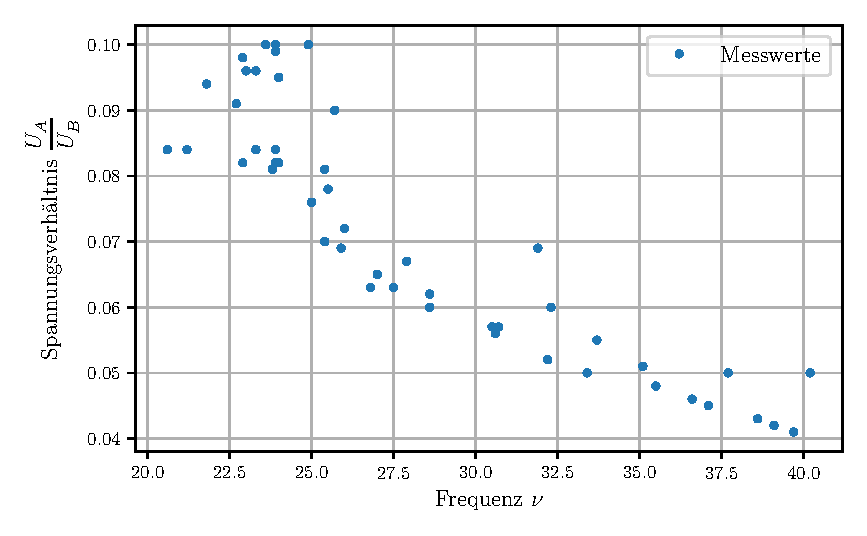
\includegraphics{content/filterkurvePLOT.pdf}
  \caption{Filterkurve des Selektivverstärkers.}
\end{figure}

\subsection{Bestimmung der Suszeptibilitäten}
\label{subsec:Suszeptibilität}

Die Suszeptibilitäten $\chi$ der beiden Stoffe sollen mithilfe der Messwerte aus Tabelle \ref{tab:Messwerte} bestimmt werden.
Dabei werden die Formeln \eqref{eqn:chi_r} und \eqref{eqn:chi_u} verwendet.
In der Tabelle \ref{tab:Suszeptibilität_Praxis} sind die Ergebnisse zu finden.

\begin{table}
  \centering
  \label{tab:Messwerte}
  \begin{tabular}{c c c c c c}
    \toprule
    {Stoff} & {$U_{\text{Br ohne}}$ [$\si{\milli\volt}$]} & {$U_{\text{Br mit}}$ [$\si{\milli\volt}$]} & {$R_{3 \text{ohne}}$ [$\si{\milli\ohm}$]} &{$R_{3 \text{mit}}$ [$\si{\milli\ohm}$]} & {$\increment R_3$ [$\si{\milli\ohm}$]}\\
    \midrule
    $\ce{Dy2O3}$ & 0.09 & 0.370 & 2964.5 & 1690.0 & 1274.5\\
              &0.13 & 0.392 & 2981.0 & 1530.0 & 1451.0\\
              &0.12 & 0.420 & 3059.0 & 1485.5 & 1574.0\\
    $\ce{Gd2O3}$ &0.20 & 0.405 & 3136.5 & 2360.0 & 776.5\\
              &0.21 & 0.407 & 3157.5 & 2398.0 & 759.5\\
              &0.21 & 0.385 & 3137.0 & 2381.0 & 756.0\\
    \bottomrule
  \end{tabular}
  \caption{Messergebnisse zur Bestimmung der Suszeptibilitäten.}
\end{table}

\begin{table}
  \centering
  \label{tab:Suszeptibilität_Praxis}
  \begin{tabular}{c c c}
    \toprule
    {Stoff} & {$\chi_U$} & {$\chi_R$} \\
    \midrule
    $\ce{Dy2O3}$ & 0.00867 $\pm$ 0.00029 & 0.02218 $\pm$ 0.00110 \\
    $\ce{Gd2O3}$ & 0.00607 $\pm$ 0.00023 & 0.01217 $\pm$ 0.00008 \\
    \bottomrule
  \end{tabular}
  \caption{Suszeptibilitäten aus den Messergebnissen.}
\end{table}
\noindent
Die Suszeptibilitäten aus den Messergebnissen werden mit dem Theoriewert verglichen.
Dieser wird mithilfe der Formel \eqref{eqn:sus_theo} bestimmt.
Das in dieser Formel genutzte $N$ berechnet sich nach
\begin{equation*}
  N = z \cdot \frac{N_{\text{A}} \rho_{\text{w}}}{M},
\end{equation*}
wobei hier $z = \num{2}$ gilt und $N_{\text{A}}$ die Avogadro-Konstante bezeichnet.
In Tabelle \ref{tab:Proben} ist jeweils die Dichte $\rho$, Masse $m$, Länge $l$, molare Masse $M$ und der reale Querschnitt $Q$ der beiden Proben zu finden, die für die Berechnung benötigt werden.
Der reale Querschnitt $Q$ wird mit der Formel \eqref{eqn:qreal} ermittelt.

\begin{table}
  \centering
  \label{tab:Proben}
  \begin{tabular}{c c c c c c }
    \toprule
    {Stoff} & {$\rho$ [$\si{\gram\per\centi\metre\cubed}$]} & {$m$ [$\si{\gram}$]} & {$l$ [$\si{\centi\metre}$]} & {$M$ [$\si{\gram\per\mole}$]} & {$Q$ [$\si{\centi\metre\squared}$]}\\
    \midrule
    $\ce{Dy2O3}$ & 7.8 & 15.1 & 17.3 & 372.9982 & 0.1119\\
    $\ce{Gd2O3}$ & 7.4 & 14.08 & 17.5 & 362.4982 & 0.1087\\
    \bottomrule
  \end{tabular}
  \caption{Werte der Proben.}
\end{table}

\begin{table}
  \centering
  \begin{tabular}{c c c c c }
    \toprule
    {Stoff} & {$L$} & {$S$} & {$J$} & {$g_J$}\\
    \midrule
    $\ce{Dy2O3}$ & 5 & 2.5 & 7.5 & 1.33\\
    $\ce{Gd2O3}$ & 0 & 3.5 & 3.5 & 2.0\\
    \bottomrule
  \end{tabular}
  \caption{Quantenzahlen und Landé-Faktoren.}
\end{table}

\begin{table}
  \centering
  \label{tab:vergleich}
  \begin{tabular}{c c c c c c}
    \toprule
    {Stoff} & {$\chi_T$} &{$\chi_U$} & {$\frac{\chi_T - \chi_U}{\chi_T}$} & {$\chi_R$} & {$\frac{\chi_T - \chi_R}{\chi_T}$}\\
    \midrule
    $\ce{Dy2O3}$ & 0.02569 & 0.00867 $\pm$ 0.00029 & 0.6625 & 0.02218 $\pm$ 0.00110 & 0.1364 \\
    $\ce{Gd2O3}$ & 0.01394 & 0.00607 $\pm$ 0.00023 & 0.5641 & 0.01217 $\pm$ 0.00008 & 0.1269 \\
    \bottomrule
  \end{tabular}
  \caption{Vergleich der Suszeptibilitäten.}
\end{table}